\subsection{Protocolo HTTP}

El Protocolo de transferencia de hipertexto (HTTP) es un protocolo de 
solicitud/respuesta “stateless” (sin estado) que utiliza semántica 
extensible y cargas útiles de mensajes autodescriptivos para una 
interacción flexible con sistemas basados en red.
   HTTP es un protocolo genérico para sistemas de información. Está 
   diseñado para ocultar los detalles de cómo se implementa un servicio 
   mostrando una interfaz a los clientes que es independiente de los 
   tipos de recursos proporcionados. Del mismo modo, los servidores 
   no necesitan conocer el propósito de cada cliente: una solicitud 
   HTTP puede aislada en vez de estar asociada con un tipo específico
    de cliente o una secuencia predeterminada de pasos de la aplicación.
     El resultado es un protocolo que se puede utilizar de forma eficaz 
     en muchos contextos diferentes y cuyas implementaciones pueden
      evolucionar a lo largo del tiempo.
   Una consecuencia de esta flexibilidad es que el protocolo no 
   se puede definir en términos de lo que ocurre detrás de la 
   interfaz: estamos limitados a definir la sintaxis de la comunicación, 
   los mensajes y el comportamiento esperado de los destinatarios. 
   Si la comunicación se considera de forma aislada, las acciones 
   exitosas deben reflejarse correspondientemente. Sin embargo, 
   dado que varios clientes pueden actuar en paralelo y quizás con
    propósitos cruzados, no podemos exigir que tales cambios sean 
    observables más allá del alcance de una única respuesta.
   
\subsection{Arquitectura}
HTTP fue creado para la arquitectura World Wide Web (WWW) y ha 
evolucionado con el tiempo para soportar las necesidades de
 escalabilidad de un sistema mundial. Gran parte de esa arquitectura 
 se refleja en la terminología y  definiciones de sintaxis utilizadas 
 para definir HTTP.

\subsubsection*{Mensajes Cliente/Servidor}


HTTP es un protocolo de solicitud/respuesta que opera intercambiando 
mensajes a través de una ``conexión'' en la capa de sesión o transporte.
 Un "cliente" HTTP es un programa que establece una conexión a un 
 servidor con el propósito de enviar una o más solicitudes HTTP. 
 Un "servidor" HTTP es un programa que acepta conexiones para
  atender solicitudes HTTP mediante el envío de respuestas HTTP. 
  La mayoría de las comunicaciones HTTP consisten en una solicitud
   (GET) de algún recurso identificado por un URI. En el caso más 
   simple, esto podría lograrse mediante una única conexión entre un
    usuario y el servidor.

\begin{center}
   \begin{figure}   
      \begin{center}
         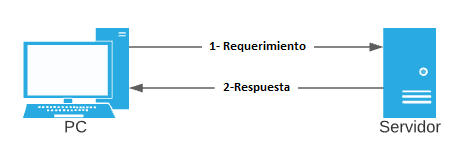
\includegraphics{2.1.png}
      \end{center}
      \caption{Comunicación básica en HTTP}
   \end{figure}
\end{center}

Un cliente envía una solicitud HTTP a un servidor en forma de mensaje
 de solicitud, comenzando con una línea que incluye un método, URI y 
 versión del protocolo, seguida de campos de encabezado que contienen
  modificadores de solicitud, información del cliente y metadatos de
   representación, una línea vacía para indicar el final de la sección
    del encabezado, y finalmente un cuerpo del mensaje que contiene el 
    cuerpo de la carga útil (si lo hay). Un servidor responde a la 
    solicitud de un cliente enviando uno o más mensajes de respuesta 
    HTTP, cada uno de los cuales comienza con una línea de estado que 
    incluye la versión del protocolo, un código de estado (éxito o error)
     y una descripción en forma de texto asociada al mismo, posiblemente 
     seguida de campos de encabezado con información del servidor y
      metadatos de recursos, una línea vacía para indicar el final 
      de la sección del encabezado y finalmente, un cuerpo del mensaje
       la carga útil del mismo

\subsubsection*{Ejemplo}
El siguiente ejemplo ilustra un intercambio de mensajes típico 
para una solicitud GET a la direccion "http://www.example.com/hello.txt":

\bigskip
\noindent
\underline{Client request:}
\begin{verbatim}
   GET /hello.txt HTTP/1.1
   User-Agent: curl/7.16.3 libcurl/7.16.3 OpenSSL/0.9.7l zlib/1.2.3
   Host: www.example.com
   Accept-Language: en, mi
  \end{verbatim}
\underline{Server response:}
\begin{verbatim}
   HTTP/1.1 200 OK
   Date: Mon, 27 Jul 2009 12:28:53 GMT
   Server: Apache
   Last-Modified: Wed, 22 Jul 2009 19:15:56 GMT
   ETag: "34aa387-d-1568eb00"
   Accept-Ranges: bytes
   Content-Length: 51
   Vary: Accept-Encoding
   Content-Type: text/plain

   Hello World! My payload includes a trailing CRLF.
\end{verbatim}


\subsection{Métodos mas importantes del del protocolo HTTP}

El protocolo HTTP contiene varios método, comopor ejemplo PUT, HEAD, DELETE, etc. Sin
embargo, para nuestro trabajo explicaremos los dos mas utilizados GET y POST, lo que
nos permitirá tener una base a la hora del caso de estudio del capitulo \ref{capCaseOfStudy}

%CONNECT OPTIONS TRACE PUT 

\subsubsection*{GET}

El método GET solicita al servidor la transferencia de un recurso.
GET es el mecanismo principal de recuperación de información y el 
foco de casi todas las optimizaciones de rendimiento. Por lo tanto,
cuando las personas hablan de recuperar información identificable
a través de HTTP, generalmente se refieren a realizar una solicitud
GET.

Se puede pensar que a la hora de solicitar un recuro, este sea un archivo 
dentro de un directorio, y la respuesta sea el mismo archivo. Sin embargo, 
no existen tales limitaciones en la práctica. De hecho, se puede 
configurar un servidor para ejecutar los archivos de la solicitud y 
enviar la salida en lugar de transferir los archivos directamente. 
Independientemente de la solicitud, el servidor solo necesita saber 
cómo tratar a cada uno de sus recursos.

\subsubsection*{POST}

El método POST solicita que un recurso del servidor sea procesado con 
los datos que el cliente le envía. Por ejemplo, POST se utiliza para 
las siguientes funciones (entre otras):

\begin{itemize}
   \item Proporcionar un bloque de datos, como los campos ingresados 
   en un formulario HTML, a un proceso de manejo de datos.
   \item Publicar un mensaje en un tablón de anuncios, grupo de 
   noticias, lista de correo, blog o grupo similar de artículos.
   \item Crear un nuevo recurso que aún no ha sido identificado por 
   el servidor.
   \item Agregar datos a las representaciones existentes de un recurso.
\end{itemize}


\subsection{Response Status Codes} 
El código de estado es un número entero de tres dígitos que da el 
resultado del intento de comprender y satisfacer la solicitud.

   Los códigos de estado HTTP son extensibles. No se requiere que los
    clientes HTTP comprendan el significado de todos los códigos de
     estado registrados, aunque se espara una mínima comprensión.

   Por ejemplo, si un cliente recibe un código de estado no reconocido
    de 471, el cliente puede asumir que hubo algo mal con su solicitud
     y tratar la respuesta como si hubiera recibido un código de estado
      400 (Solicitud incorrecta). El mensaje de respuesta generalmente 
      contendrá una representación que explica el estado.

   El primer dígito del código de estado define la clase de respuesta.
    Los dos últimos dígitos no tienen ninguna función de categorización.
     Hay cinco valores para el primer dígito:

   o 1xx (Informativo): Se recibió la solicitud, se continua procesando

   o 2xx (satisfactoria): la solicitud se recibió, comprendió y 
   aceptó correctamente

   o 3xx (redireccionamiento): se deben realizar más acciones para
    completar la solicitud

   o 4xx (Error del cliente): la solicitud contiene una sintaxis
    incorrecta o no se puede cumplir

      o 5xx (error del servidor): el servidor no cumplió con una
       solicitud aparentemente válida


\subsection{HTTPS con SSL} 

Con una comprensión mínima de los conceptos la criptografía, podemos 
observar cómo funciona el protocolo Secure Sockets Layer (ssl). Aunque
 ssl no es un protocolo extremadamente complicado, ofrece varias 
 opciones y variaciones.

El protocolo ssl consiste en un conjunto de mensajes y reglas sobre
 cuándo enviar (y no enviar) cada mensaje. En este capítulo, consideramos 
 cuáles son esos mensajes, la información general que contienen y 
 cómo los sistemas usan los diferentes mensajes en una sesión de
  comunicaciones.


\subsubsection*{SSL Roles}
El protocolo Secure Sockets Layer define dos roles diferentes para las
partes que se comunican. Por un lado tenemos un cliente, y por el otro
un servidor. La distinción es muy importante, porque ssl requiere que 
los dos sistemas se comporten de manera muy diferente. 

El cliente es el sistema que inicia las comunicaciones seguras; el 
servidor responde a la solicitud del cliente. En el uso más común 
de ssl, la navegación web segura, el navegador web es el cliente ssl 
y el sitio web es el servidor ssl. Para SSL en sí, las distinciones 
más importantes entre clientes y servidores son sus acciones durante 
la negociación de los parámetros de seguridad.

Dado que el cliente inicia una comunicación, tiene la responsabilidad 
de proponer un conjunto de opciones ssl para usar en el intercambio. 
El servidor selecciona entre las opciones propuestas por el cliente 
y decide qué utilizarán realmente los dos sistemas. Aunque la decisión 
final recae en el servidor, el servidor solo puede elegir entre las 
opciones que el cliente propuso originalmente.


\subsubsection*{Mensajes SSL}
Cuando los clientes y servidores ssl se comunican, lo hacen 
intercambiando mensajes ssl. Este capítulo mostrará cómo los 
sistemas utilizan estos mensajes en sus comunicaciones. La función 
más básica (y uno de los propósitos mas importantes) que realiza 
un cliente y un servidor SSL es establecer la seguridad a través
de un canal para comunicaciones cifradas. Los primeros tres mensajes
SYN, SYN ACK y SYN corresponden al protocolo TCP, Luego, inician los 
mensajes pertenecientes a la comunicación SSL.


\begin{center}
   \begin{figure}   
      \begin{center}
         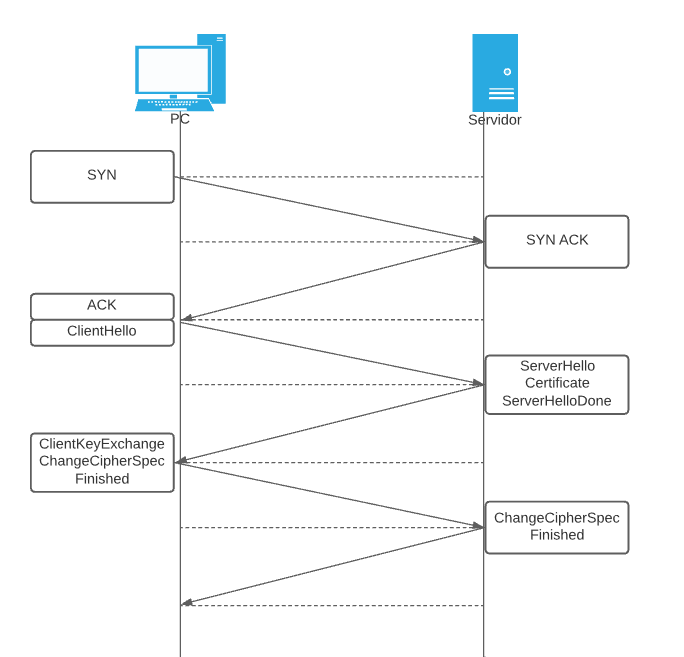
\includegraphics[width=13cm,height=13cm]{2.2.5.png}
      \end{center}
      \caption{Mensajes SSL (grafico beta)}
   \end{figure}
\end{center}


\paragraph*{ClientHello}
El mensaje ClientHello inicia la comunicación ssl entre las dos partes. 
El cliente usa este mensaje para pedirle al servidor que comience a 
negociar los servicios de seguridad usando ssl.

El mensaje este compuesto por ciertos campos: 
\begin{itemize}
   \item Versión: refiere a la versión más alta de SSL que el cliente 
   puede admitir. 
   \item RandomNumber: proporciona la semilla para cálculos criptográficos
   críticos. 
   \item SessionID: es opcional, y muchas veces no es utilizado. 
   \item CipherSuites: permite a un cliente enumerar los diversos 
   servicios criptográficos que el cliente puede admitir
   \item CompressionMethods: es utilizado por el cliente para enumerar 
   todos los diversos métodos de compresión de datos que puede admitir.
    Los métodos de compresión son una parte importante de ssl porque el 
    cifrado tiene una secuencia significativa en la efectividad de 
    cualquier técnica de compresión de datos. 
\end{itemize}


\paragraph*{ServerHello}
Cuando el servidor recibe el mensaje ClientHello, responde con un 
"ServerHello". En este mensaje el servidor toma la decisión de elegir 
la versión de SSL que se utilizará, además se establece un SessionID, 
que identifica de forma única esta sesión o comunicación SSL en particular. 
La razón principal para identificar explícitamente una sesión SSL en 
particular es hacer referencia a ella en mensajes posteriores. Por 
último, se establece los parámetros criptográficos y mecanismos de 
compresión a utilizar. Cade aclarar que, las versiones actuales de 
SSL no han definido ningún método de compresión, por lo que este 
campo no tiene ninguna utilidad práctica.

\paragraph*{ServerKeyExchange}
In this example, the server follows its ServerHello message with a
ServerKeyExchange message. This message complements the CipherSuite field 
of the ServerHello. While the CipherSuite field indicates
the cryptographic algorithms and key sizes, this message contains the
public key information itself. The exact format of the key information depends
 on the particular public key algorithm used. For the rsa
algorithm, for example, the server includes the modulus and public
exponent of the server’s rsa public key.
Note that the ServerKeyExchange message is transmitted without
encryption, so that only public key information can be safely included within it.
 The client will use the server’s public key to encrypt
a session key, which the parties will use to actually encrypt the application
 data for the session.
\paragraph*{ServerHelloDone}
The ServerHelloDone message tells the client that the server has finished with
 its initial negotiation messages. The message itself contains no other 
 information, but it is important to the client, because
once the client receives a ServerHelloDone, it can move to the next
phase of establishing the secure communications.
\paragraph*{ClientKeyExchange}
When the server has finished its part of the initial ssl negotiation,
the client responds with a ClientKeyExchange message. Just as the
ServerKeyExchange provides the key information for the server, the
ClientKeyExchange tells the server the client’s key information. In

this case, however, the key information is for the symmetric encryption 
algorithm both parties will use for the session. Furthermore, the
information in the client’s message is encrypted using the public key
of the server. This encryption protects the key information as it traverses
 the network, and it allows the client to verify that the server
truly possesses the private key corresponding to its public key. Otherwise,
 the server won’t be able to decrypt this message. This operation is an 
 important protection against an attacker that intercepts
messages from a legitimate server and pretends to be that server by
forwarding the messages to an unsuspecting client. Since a fake
server won’t know the real server’s private key, it won’t be able to decrypt 
the ClientKeyExchange message. Without the information in
that message, communication between the two parties cannot succeed.
\paragraph*{ChangeCipherSpec}
After the client sends key information in a ClientKeyExchange message, 
the preliminary ssl negotiation is complete. At that point, the
parties are ready to begin using the security services they have negotiated.
 The ssl protocol defines a special message—
ChangeCipherSpec—to explicitly indicate that the security services
should now be invoked.
Since the transition to secured communication is critical, and both
parties have to get it exactly right, the ssl specification is very precise
in describing the process. First, it identifies the set of information
that defines security services. That information includes a specific
symmetric encryption algorithm, a specific message integrity algorithm, 
and specific key material for those algorithms. The ssl specification also 
recognizes that some of that information (in particular,
the key material) will be different for each direction of communication. 
In other words, one set of keys will secure data the client sends
to the server, and a different set of keys will secure data the server
sends to the client. (In principle, the actual algorithms could differ as
well, but ssl does not define a way to negotiate such an option.) For
any given system, whether it is a client or a server, ssl defines a write
state and a read state. The write state defines the security information

for data that the system sends, and the read state defines the security
information for data that the system receives.
The ChangeCipherSpec message serves as the cue for a system to
begin using its security information. Before a client or server sends a
ChangeCipherSpec message, it must know the complete security information it 
is about to activate. As soon as the system sends this
message, it activates its write state. Similarly, as soon as a system receives
 a ChangeCipherSpec from its peer, the system activates its
read state.

GRAFIQUITO Figures 3-2 and 3-3

\paragraph*{Finished}
Immediately after sending their ChangeCipherSpec messages, each
system also sends a Finished message. The Finished messages allow
both systems to verify that the negotiation has been successful and
that security has not been compromised. Two aspects of the Finished
message contribute to this security. First, as the previous subsection
explained, the Finished message itself is subject to the negotiated cipher suite. 
That means that it is encrypted and authenticated according to that suite.
 If the receiving party cannot successfully decrypt
and verify the message, then clearly something has gone awry with
the security negotiation.
The contents of the Finished message also serve to protect the security of the
 ssl negotiation. Each Finished message contains a cryptographic hash of 
 important information about the just-finished
negotiation.  Notice that protected data includes the exact content of all
handshake messages used in the exchange (though ChangeCipherSpec messages 
are not considered “handshake” messages in the strict
sense of the word, and thus are not included). This protects against
an attacker who manages to insert fictitious messages or remove 
legitimate messages from the communication. If an attacker were able
to do so, the client’s and server’s hash calculations would not match,
and they would detect the compromise.

\paragraph*{Ending Secure Communications}

Although as a practical matter it is rarely used (primarily due to the
nature of Web sessions), ssl does have a defined procedure for ending a
 secure communication between two parties. In this procedure,
 the two systems each send a special ClosureAlert to the other.
Explicitly closing a session protects against a truncation attack, in
which an attacker is able to compromise security by prematurely terminating
 a communication. 

\subsubsection*{Authenticating the Server’s Identity}
previously it was explained how ssl can establish encrypted
communications between two parties, that may not really add that
much security to the communication. With encryption alone neither
party can really be sure of the other’s identity. The typical reason for
using encryption in the first place is to keep information secret from
some third party. But if that third party were able to successfully
masquerade as the intended recipient of the information, then encryption 
would serve no purpose. The data would be encrypted, but
the attacker would have all the data necessary to decrypt it.
To avoid this type of attack, ssl includes mechanisms that allow each
party to authenticate the identity of the other. With these mechanisms, 
each party can be sure that the other is genuine, and not a
masquerading attacker. In this section, we’ll look at how ssl enables a
server to authenticate itself.
A natural question is, of course, if authenticating identities is so important,
 why don’t we always authenticate both parties? 
 Aca un ejemplo que sirva en una red interna
 The answer
lies in the nature of Web commerce. When you want to purchase
something using your Web browser, it’s very important that the Web
site you’re browsing is authentic. You wouldn’t want to send your
credit card number to some imposter posing as your favorite merchant. 
The merchant, on the other hand, has other means for
authenticating your identity. Once it receives a credit card number,
for example, it can validate that number. Since the server doesn’t
need ssl to authenticate your identity, the ssl protocol allows for
server authentication only. 

\paragraph*{Certificate}
When authenticating your identity, the server sends a Certificate message 
in place of the ServerKeyExchange message previously described. The Certificate 
message simply contains a certificate chain
that begins with the server’s public key certificate and ends with the
certificate authority’s root certificate.
The client has the responsibility to make sure it can trust the certificate it 
receives from the server. That responsibility includes verifying
the certificate signatures, validity times, and revocation status. It also
means ensuring that the certificate authority is one that the client
trusts. Typically, clients make this determination by knowing the
public key of trusted certificate authorities in advance, through some
trusted means. Netscape and Microsoft, for example, preload their
browser software with public keys for well-known certificate authorities. 
Web servers that want to rely on this trust mechanism can only
obtain their certificates (at least indirectly) from one of these wellknown
 authorities.

\paragraph*{ClientKeyExchange}
The client’s ClientKeyExchange message also differs in server authentication, 
though the difference is not major. When encryption
only is to be used, the client encrypts the information in the ClientKeyExchange
 using the public key the server provides in its
ServerKeyExchange message. In this case, of course, the server is authenticating
 itself and, thus, has sent a Certificate message instead of
a ServerKeyExchange. The client, therefore, encrypts its ClientKeyExchange information 
using the public key contained in the
server’s certificate. This step is important because it allows the client
to make sure that the party with whom it is communicating actually
possesses the server’s private key. Only a system with the actual private key will 
be able to decrypt this message and successfully continue the communication.

\subsubsection*{Certificate Functionality}

\paragraph*{Single Domain}
As the name suggests, a single domain SSL certificate can only be used on a single 
domain or IP. This is considered the default SSL certificate type. The DV SSL type is
available at all validation levels.
\paragraph*{Multi-Domain}
This SSL type is a jack-of-all-trades certificate. Multi-Domain Wildcards can encrypt
 up to 250 different domains and unlimited sub-domains. Unfortunately, it's not available
  in EV.
\paragraph*{Wildcard}
Wildcards are specifically designed to encrypt one domain and all of its accompanying 
sub-domains. Unlimited sub-domains. Unfortunately, Wildcards are only available at the 
DV and OV levels.
\paragraph*{Multi-Domain Wildcard}
These are the jack-of-all-trades certificates. Multi-Domain Wildcards can encrypt up 
to 250 different domains and unlimited sub-domains. Unfortunately, it's not available 
in EV.

\subsubsection*{Validation Level}
There are three types of SSL Certificate available today; Extended Validation 
(EV SSL), Organization Validated (OV SSL) and Domain Validated (DV SSL). The 
encryption levels are the same for each certificate, what differs is the vetting
 and verification processes needed to obtain the certificate.
\paragraph*{Domain Validation (DV)}
Domain Validation SSL or DV SSL represents the base-level for SSL types. These 
are perfect for websites that just need encryption and nothing more. DV SSL 
certificates are typically inexpensive and they can be issued within minutes. That's 
because the validation process is fully automated. Just prove you own your domain 
and the DV SSL certificate is yours.
\paragraph*{Organization Validation (OV)}
Organization Validation SSL or OV SSL represents the middle ground for SSL certificate 
types. To obtains OV SSL, your company or organization must undergo light business
 vetting. This can take up to three business days because someone has to verify 
 your business information. OV SSL displays the same visual indicators as DV SSL,
  but provides a way for your customers to check your verified business information 
  in the certificate details section.
\paragraph*{Extended Validation (EV)}
Extended Validation SSL or EV SSL requires extensive business vetting by Comodo. This
 may sound like a lot, but it's really not if your business has publicly available 
 records. EV SSL activates a unique visual indicator – your verified organization name
  shown in the browser.

  
\subsubsection*{Identifier Validation Challenges}

(CAMBIAR LA INTRO, NO ME GUSTA LO DE IDENTIFICADOR, RELACIONARLO MAS CON UN DOMINIO)

ACME uses an extensible challenge/response framework for identifier
validation.  The server presents a set of challenges in the
authorization object it sends to a client (as objects in the
"challenges" array), and the client responds by sending a response
object in a POST request to a challenge URL.

   Different challenges allow the server to obtain proof of different
   aspects of control over an identifier.  In some challenges, like HTTP
   and DNS, the client directly proves its ability to do certain things
   related to the identifier.  The choice of which challenges to offer
   to a client under which circumstances is a matter of server policy.


   

\paragraph*{HTTP Challenge}

   With HTTP validation, the client in an ACME transaction proves its
   control over a domain name by proving that it can provision HTTP
   resources on a server accessible under that domain name.  The ACME
   server challenges the client to provision a file at a specific path,
   with a specific string as its content.

   This is the most common challenge type today. The server gives a
   token to your ACME client, and your ACME client puts a file on your web 
   server at {http://\<YOUR\_DOMAIN\>/.well-known/acme-challenge/\<TOKEN\>}. That 
   file contains the token, plus a thumbprint of your account key. 

   Once the client tells to the server that the file is ready, the server 
   tries retrieving it.On receiving a response, the server constructs and stores the key
   authorization from the challenge "token" value and the current client
   account key.

   Given a challenge/response pair, the server verifies the client's
   control of the domain by verifying that the resource was provisioned
   as expected.

   (TAL VEZ PARA LA PRESENTACION)

   Pros:

    It’s easy to automate without extra knowledge about a domain’s configuration.
    It allows hosting providers to issue certificates for domains CNAMEd to them.
    It works with off-the-shelf web servers.

   Cons:

    It doesn’t work if your ISP blocks port 80 (this is rare, but some residential ISPs do this).
    Let’s Encrypt doesn’t let you use this challenge to issue wildcard certificates.
    If you have multiple web servers, you have to make sure the file is available on all of them.

   (EXPLICAR POR QUE NO PUEDO USAR ESTE DESAFIO)

\paragraph*{DNS Challenge}
   When the identifier being validated is a domain name, the client can
   prove control of that domain by provisioning a TXT resource record
   containing a designated value for a specific validation domain name.

   A client fulfills this challenge by constructing a key authorization
   from the "token" value provided in the challenge and the client's
   account key.  The client then computes the SHA-256 digest 
   of the key authorization.

   The record provisioned to the DNS contains the base64url encoding of
   this digest.  The client constructs the validation domain name by
   prepending the label {\_acme-challenge} to the domain name being
   validated, then provisions a TXT record with the digest value under
   that name.  For example, if the domain name being validated is
   "www.example.org", then the client would provision the following DNS
   record:
   \_acme-challenge.www.example.org. 300 IN TXT "gfj9Xq...Rg85nM"
   
   On receiving a response, the server constructs and stores the key
   authorization from the challenge "token" value and the current client
   account key.

   To validate a DNS challenge, the server performs the following steps:

   1.  Compute the SHA-256 digest of the stored key
       authorization

   2.  Query for TXT records for the validation domain name

   3.  Verify that the contents of one of the TXT records match the
       digest value

   If all of the above verifications succeed, then the validation is
   successful.  If no DNS record is found, or DNS record and response
   payload do not pass these checks, then the validation fails.

   The client SHOULD de-provision the resource record(s) provisioned for
   this challenge once the challenge is complete, i.e., once the
   "status" field of the challenge has the value "valid" or "invalid".
